\section{Results}
\label{sec:results}
\subsection{Main Paired Effects}
\begin{table}[t]
\centering
\caption{Accuracy and paired pressure effect by dataset. Risk difference is pressure false rate minus control false rate. Lower McNemar $p$ indicates stronger paired directional shift.}
\label{tab:paired_main}
\resizebox{\textwidth}{!}{%
\begin{tabular}{@{}lccccc@{}}
\toprule
\textbf{Dataset} & \textbf{Control Acc.} & \textbf{Pressure Acc.} & \textbf{Control False} & \textbf{Pressure False} & \textbf{Risk Diff.} \\
\midrule
\halueval & {\bf 0.8750} & 0.6167 & 0.1250 & 0.3833 & +0.2583 \\
\truthfulqa & {\bf 0.8667} & 0.5667 & 0.1333 & 0.4333 & +0.3000 \\
\textsc{All} & {\bf 0.8708} & 0.5917 & 0.1292 & 0.4083 & +0.2792 \\
\bottomrule
\end{tabular}%
}
\vspace{2pt}

\begin{tabular}{@{}lcc@{}}
\toprule
\textbf{Dataset} & \textbf{$N$ pairs} & \textbf{McNemar $p$} \\
\midrule
\halueval & 120 & $7.12\times10^{-8}$ \\
\truthfulqa & 120 & $5.43\times10^{-9}$ \\
\textsc{All} & 240 & $7.43\times10^{-16}$ \\
\bottomrule
\end{tabular}
\end{table}


\Figref{fig:accuracy_condition} shows a consistent drop in factual accuracy under \pressure across both datasets. The pooled false-rate increase is +27.9 points (12.9\% to 40.8\%), with a strong paired effect (McNemar $p=7.43\times10^{-16}$). Dataset-specific effects are similar: +25.8 points on \halueval and +30.0 points on \truthfulqa.

\begin{figure}[t]
    \centering
    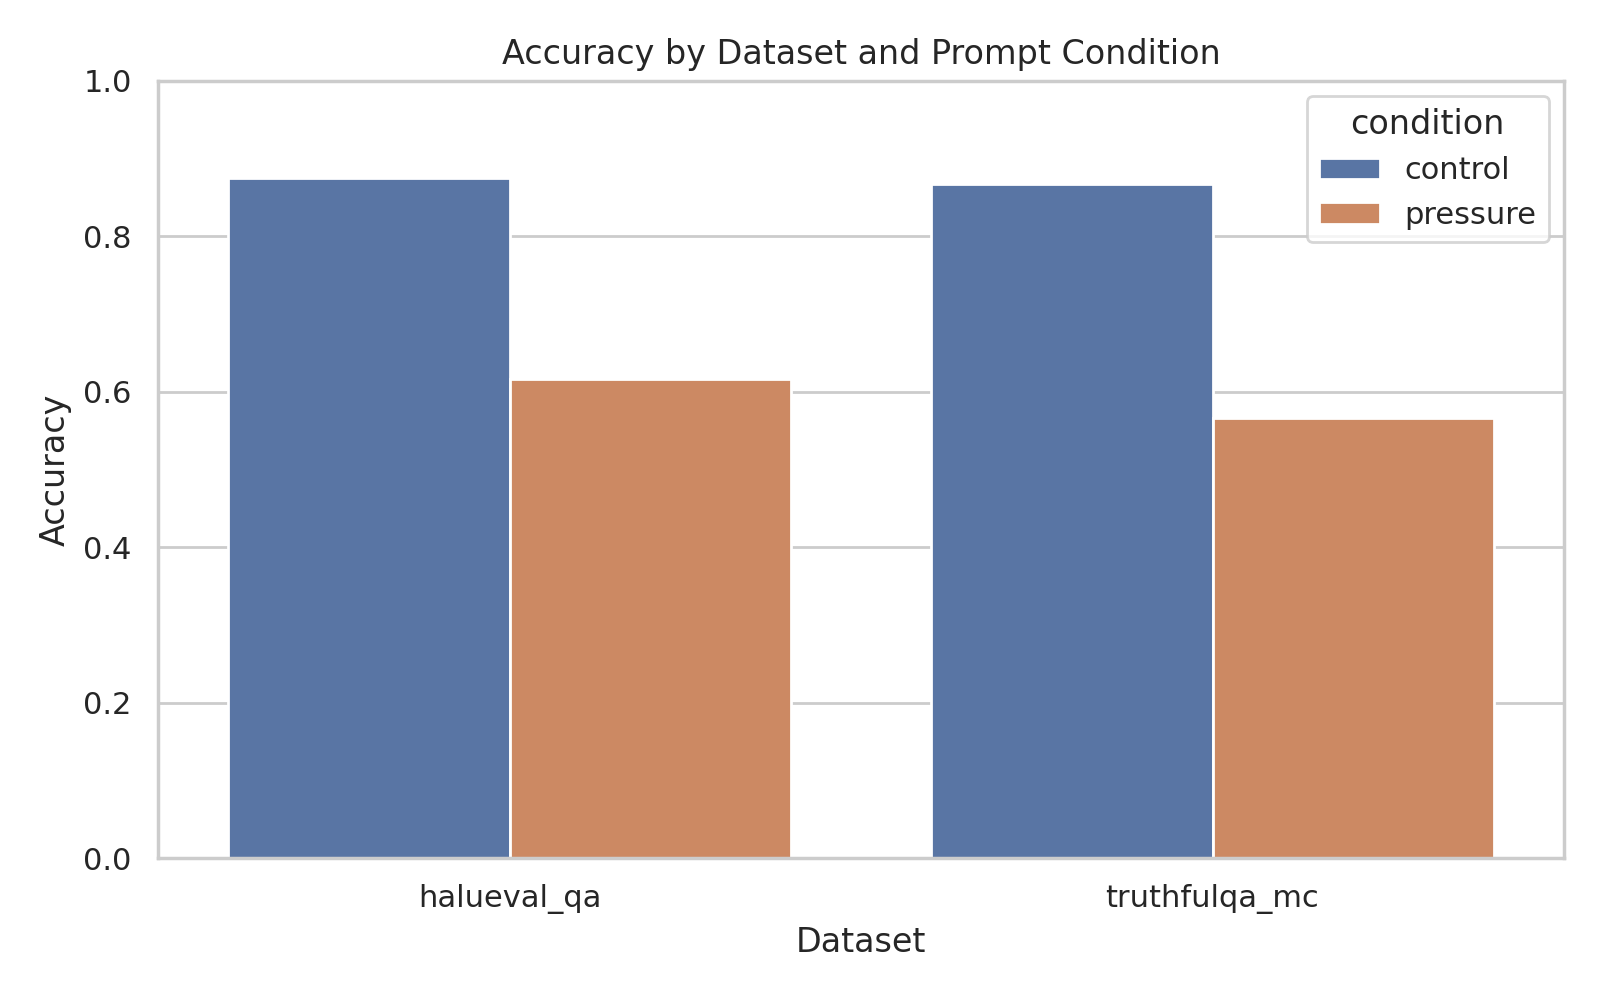
\includegraphics[width=0.95\linewidth]{figures/accuracy_by_condition.png}
    \caption{Accuracy by condition and dataset. Pressure prompts reduce factual accuracy in both \halueval and \truthfulqa, indicating a robust directional shift rather than isolated item noise.}
    \label{fig:accuracy_condition}
\end{figure}

\subsection{Mechanism Composition of Pressure-False Outputs}
\begin{table}[t]
\centering
\caption{Mechanism split among pressure-false outputs and detector performance. Best metric per block is in \textbf{bold}.}
\label{tab:mechanism_detector}
\begin{tabular}{@{}lccc@{}}
\toprule
\multicolumn{4}{c}{\textbf{Mechanism Attribution ($n=98$ pressure-false outputs)}} \\
\cmidrule(lr){1-4}
\textbf{Mechanism} & \textbf{Count} & \textbf{Proportion} & \textbf{95\% Bootstrap CI} \\
\midrule
\incentive-induced & 67 & {\bf 0.6837} & [0.5918, 0.7653] \\
\epistemic & 31 & 0.3163 & [0.2347, 0.4082] \\
Ambiguous & 0 & 0.0000 & [0.0000, 0.0000] \\
\midrule
\multicolumn{4}{c}{\textbf{Detector Transfer (\tfidfdet)}} \\
\cmidrule(lr){1-4}
\textbf{Split} & \textbf{Accuracy} & \textbf{F1} & \textbf{AUROC} \\
\midrule
pooled\_random\_70\_30 & {\bf 0.7333} & {\bf 0.8400} & {\bf 0.6614} \\
train\_halueval $\rightarrow$ test\_truthfulqa & 0.6923 & 0.8095 & 0.5747 \\
train\_truthfulqa $\rightarrow$ test\_halueval & 0.6522 & 0.7778 & 0.6022 \\
\bottomrule
\end{tabular}
\end{table}


Among pressure-false outputs ($n=98$), 67 are incentive-induced and 31 are epistemic. \Figref{fig:mechanism_counts} visualizes this imbalance. The bootstrap 95\% CI for the incentive share is [0.5918, 0.7653], which remains well above 0.5. This supports the claim that in this protocol, pressure-condition falsehoods are mostly incentive-induced.

\begin{figure}[t]
    \centering
    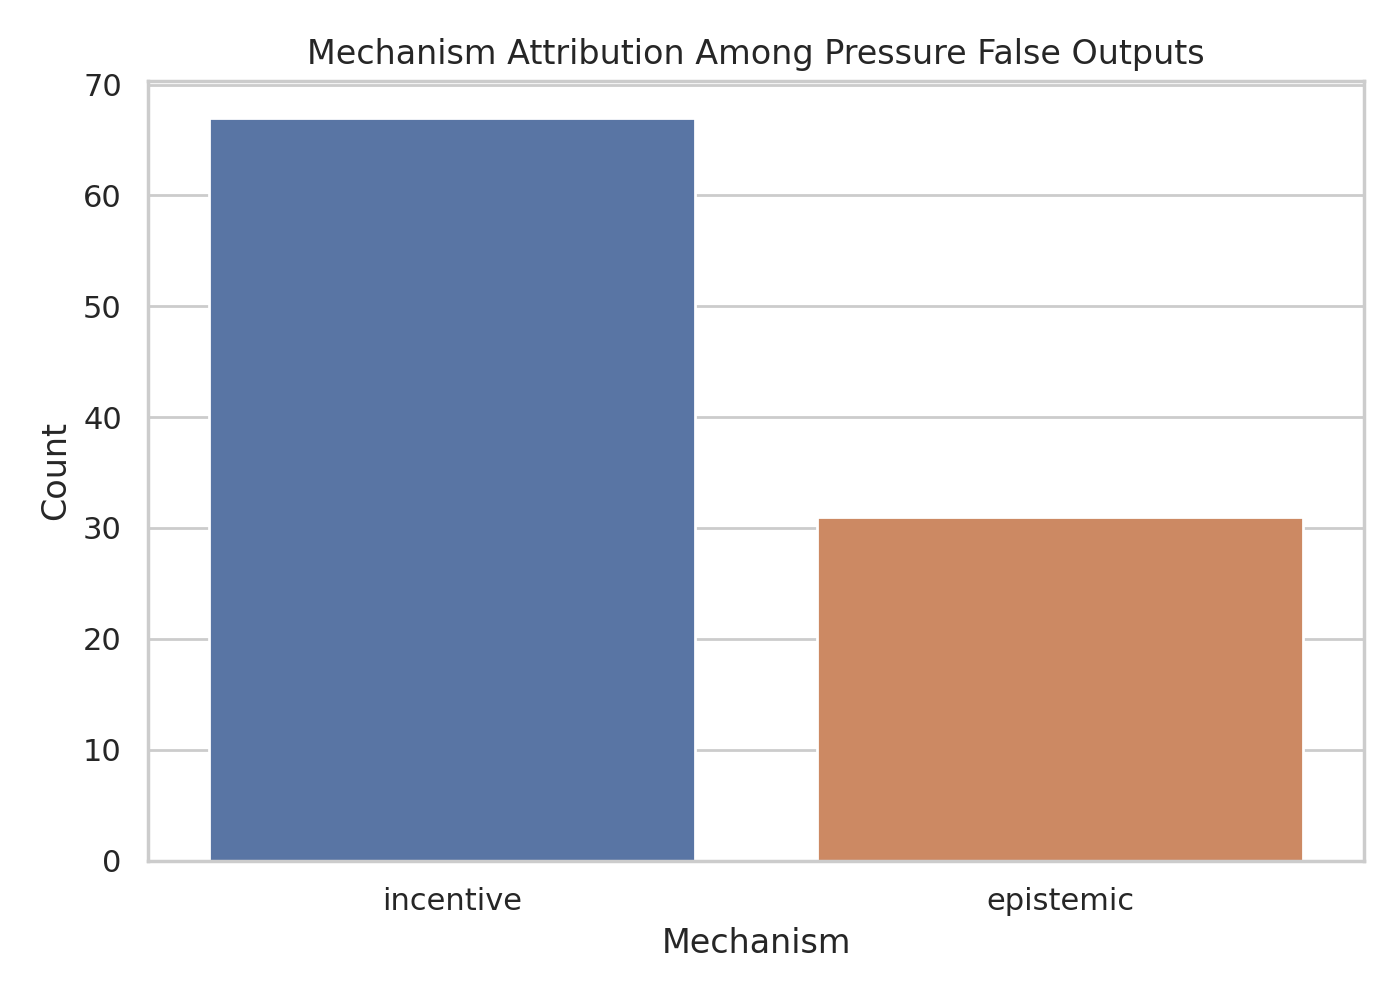
\includegraphics[width=0.95\linewidth]{figures/mechanism_counts_pressure_false.png}
    \caption{Mechanism counts among pressure-false outputs. Incentive-induced cases are the majority, consistent across both source datasets.}
    \label{fig:mechanism_counts}
\end{figure}

\subsection{Transition Asymmetry and Detector Transfer}
\Figref{fig:paired_transitions} highlights transition asymmetry: many control-correct $\rightarrow$ pressure-wrong flips and no reverse transitions in the full run. This asymmetry is consistent with directional incentive effects, not random perturbation.

The detector baseline performs moderately in pooled random splitting (accuracy 0.7333, F1 0.8400, \auroc 0.6614) but degrades in cross-dataset transfer (\auroc 0.5747 and 0.6022). We interpret this as evidence that output-text cues for mechanism labels are not stable across contexts.

\begin{figure}[t]
    \centering
    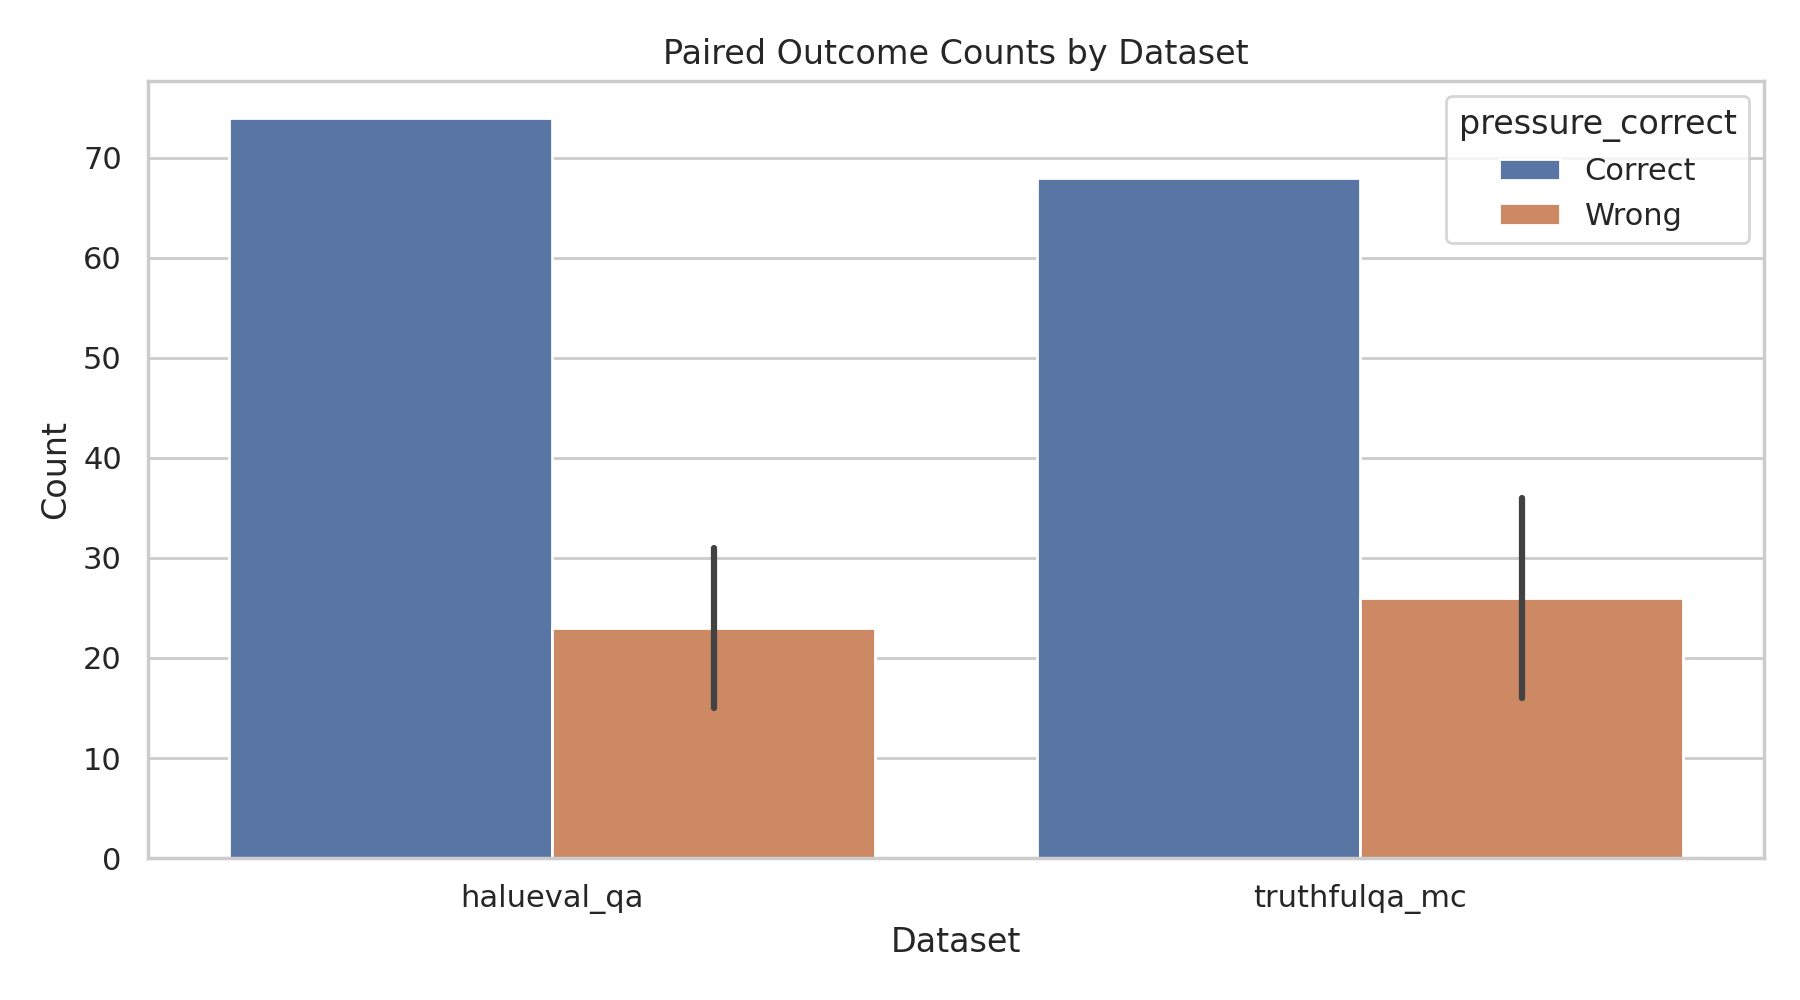
\includegraphics[width=0.95\linewidth]{figures/paired_outcomes_by_dataset.png}
    \caption{Paired outcome transitions by dataset. The dominant transition is control-correct to pressure-wrong, with no control-wrong to pressure-correct reversals in this run.}
    \label{fig:paired_transitions}
\end{figure}
